\chapter{Blur level set}
During the reconstruction of the surface all methods, in one form or another (depending on the level set computation approach), are using particle displacement information. In the SPH based fluid simulation frameworks, the displacement is usually irregular, thus small gaps can be formed. These gaps are treated as undesirable low-frequency noise. The comparison of the surface reconstruction based on a regular and irregular displacement of the particles is in Figure \ref{fig:rec_vs_displacement}.
\begin{figure}[H]
	\begin{center}
		\begin{subfigure}[b]{0.6\textwidth}
			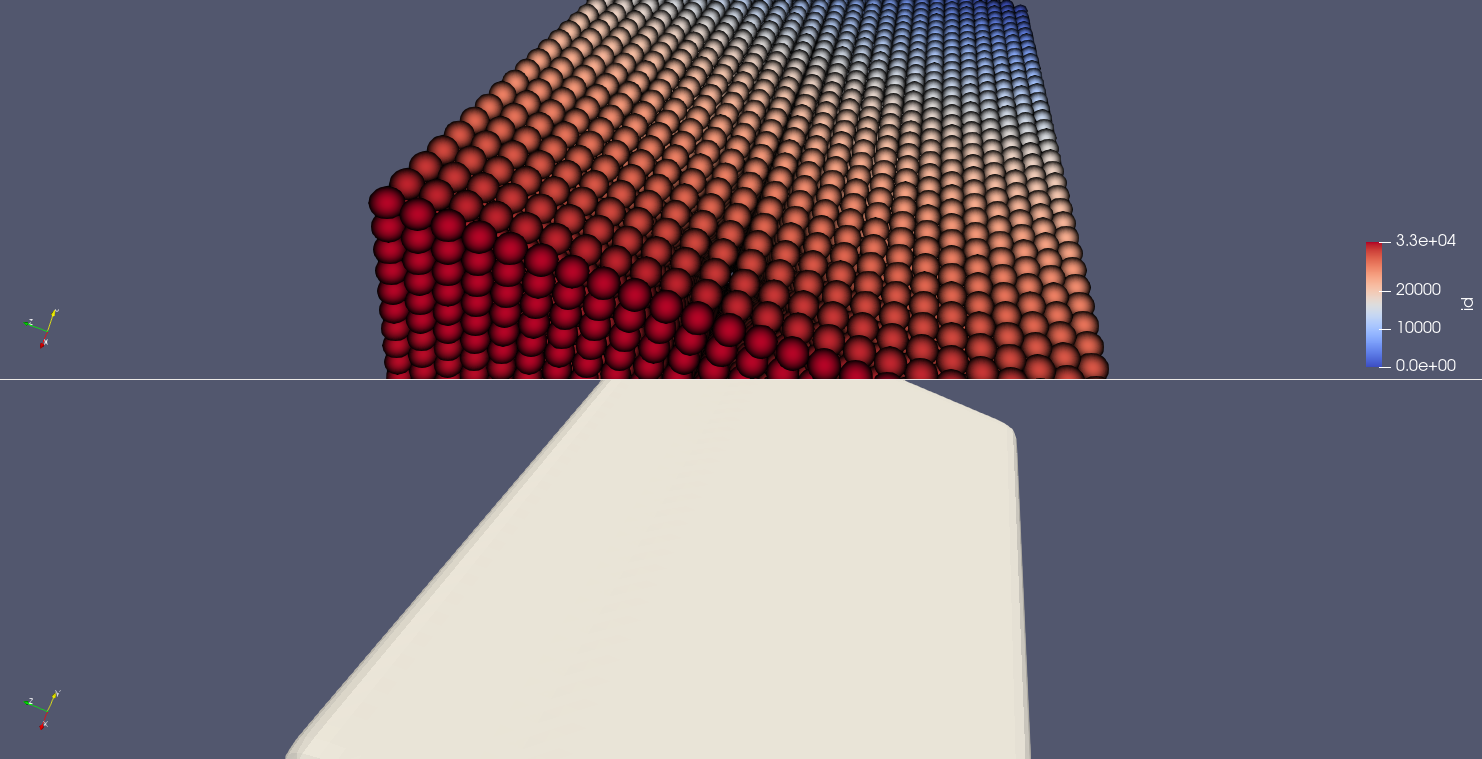
\includegraphics[width=\textwidth]{figures/FlatSurfaceWsParticleDisplacement.png}
			\caption{Regularly displaced particles}
		\end{subfigure}
		\begin{subfigure}[b]{0.6\textwidth}
			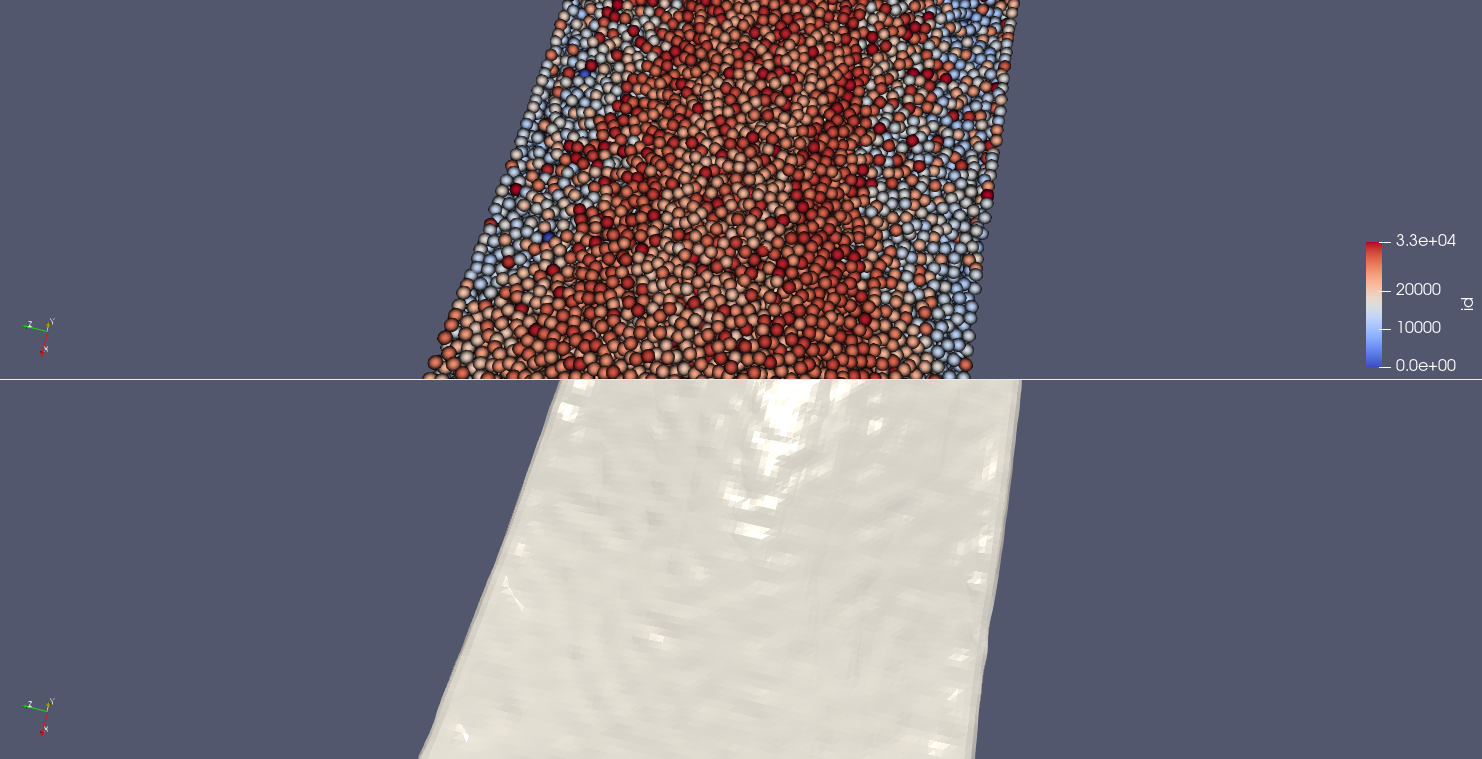
\includegraphics[width=\textwidth]{figures/NonFlatSurfaceWsParticleDisplacement.png}
			\caption{Irregularly displaced particles}
		\end{subfigure}
	\end{center}
	\caption{displacement of particles vs surface quality comparison}
	\label{fig:rec_vs_displacement}
\end{figure}
The main goal of this thesis is to develop a method, which will smooth out a high frequency bumps on flat surface areas, preserving the surface features. The first idea, that was applied to achieve this goal is simple blurring technique, which is extensively used in computer graphics, such as Gaussian Blur, Median blur, Bilateral blur or other image filtering techniques. In this chapter Blur-based method will be proposed to achieve the given goal. 
\section{Algorithm description}
Blur method was incorporated into the research framework according to the class hierarchy in Figure \ref{fig:class-diagam}. According to the class diagram, the method inherits the underlying base method (in our case its Density-Based, Zhu and Bridson, or Solenthaler methods), on top of which the computed level set is blurred.  Algorithm \ref{alg:blur_alg} shows the pseudo-code for \emph{updateLevelSet()}.
\begin{algorithm}[H]
	\scriptsize
	\begin{algorithmic}
		\State $levelSet \gets  BaseClass::initialLevelSet$
		\For{$i \in [0, blurIterations]$}
			\State blurLevelSet(levelSet);
		\EndFor
	\end{algorithmic}
	\caption{$updateLevelSet()$ for level set blurring method}
	\label{alg:blur_alg}
\end{algorithm}
According to Algorithm \ref{alg:blur_alg} blurring of the level set could be performed arbitrary number of times. The influence of number of iterations will be explained in further section.

The \emph{blurLevelSet()} pesudo-code is explained in Algorythm \ref{alg:blur_level_set}
\begin{algorithm}[H]
	\scriptsize
	\begin{algorithmic}
		\ForAll{$vtx \in MC\_CellDomain$}
			\State $neighbors \gets getNeighbourVertices(vtx);$
			\State $blurredLevelSetValue \gets 0$
			\ForAll{$nbVtx \in neighbors$}
				\State $blurredLevelSetValue\gets blurredLevelSetValue + levelSet[neighborVertex]$
			\EndFor
			\State $blurredLevelSetValue\gets\dfrac{blurredLevelSetValue}{sizeof(neighbors)}$
			\State $sf\gets computeSmoothingFactor()$
			\State $blurredLevelSet[vtx]\gets levecSet[vtx] * (1 - sf) + sf * blurredLevelSetValue;$
		\EndFor
	\end{algorithmic}
	\caption{$updateLevelSet()$ for level set blurring method}
	\label{alg:blur_level_set}
\end{algorithm}
The final blurred level set value in Algorythm \ref{alg:blur_level_set} is a wighted sum between the computed blur level set value and initial level set value.
\subsection{Smoothing factor}
The smoothing factor is a value that determines how much new, blurred level set value will contain initial level set value (weighted sum of blurred level set value and initial level set value). As described in \ref{alg:blur_level_set} level set value is updated according to the Equation \ref{eq:level_set_value}.
\begin{equation}
newLS = oldLS \cdot (1 - sf) + blurLS \cdot sf \label{eq:level_set_value}
\end{equation}
In Equation \ref{eq:level_set_value} $sf$ is a smoothing factor or a weight. The smoothing factor itself is calculated according to equation \ref{eq:smooth_factor}.
\begin{equation}
	sf_{vtx} = 1 - (1 - min(1, \dfrac{bsf \cdot fp_{vtx}}{maxFp})^2)^{10} \label{eq:smooth_factor}
\end{equation}
where:
\begin{conditions}
	vtx & vertex for which the smoothing factor is computed\\
	fp_{vtx} & number of neighbor fluid particles within support radius from vtx\\
	maxFp & maximum possible fluid particles that can be in the neighborhood of the vertex \\
	bsf & base support factor (use defined)
\end{conditions}
The smoothing factor formula was designed such that it should be maximal for vertices that contains full fluid particles set and minimum where number of fluid particles limits to zero (see Figure \ref{fig:sf_function_graph}).
\begin{figure}[H]
	\begin{center}
			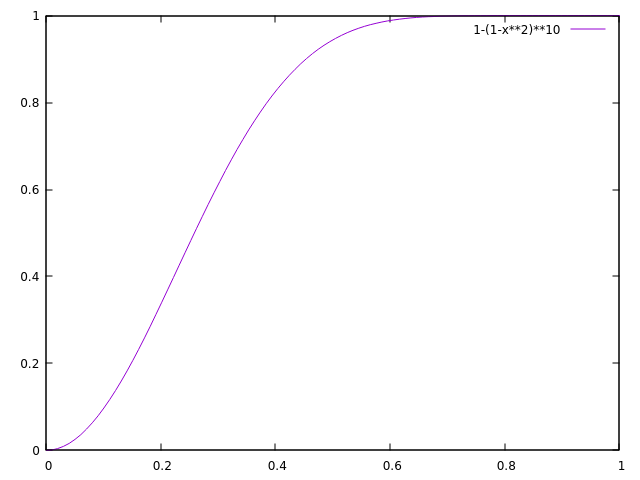
\includegraphics[width=0.5\textwidth]{figures/sf_function_graph.png}		
	\end{center}
	\caption{Graphic of function, representing equation \ref{eq:smooth_factor}. Taking into account that $min(1, \dfrac{bsf \cdot fp_{vtx}}{maxFp}) \in [0,1]$ the function converges from 0 to 1 in the interval $x \in [0, 0.5]$ and limits to 1 for the area $x\in [0.5, 1]$}
	\label{fig:sf_function_graph}
\end{figure}


The motivation to apply such a smoothing factor comes from the problem of the blurring algorithm. If we apply the blur algorithm uniformly into all MC vertex domains, the blur will smooth out the features in thin areas and the areas with a small set of particles (droplets or splashes). Figure \ref{fig:smoothing_factor_influence} shows the problem of application of the blur algorithm w.o. application of smoothing factor.

\begin{figure}[H]
	\begin{center}
			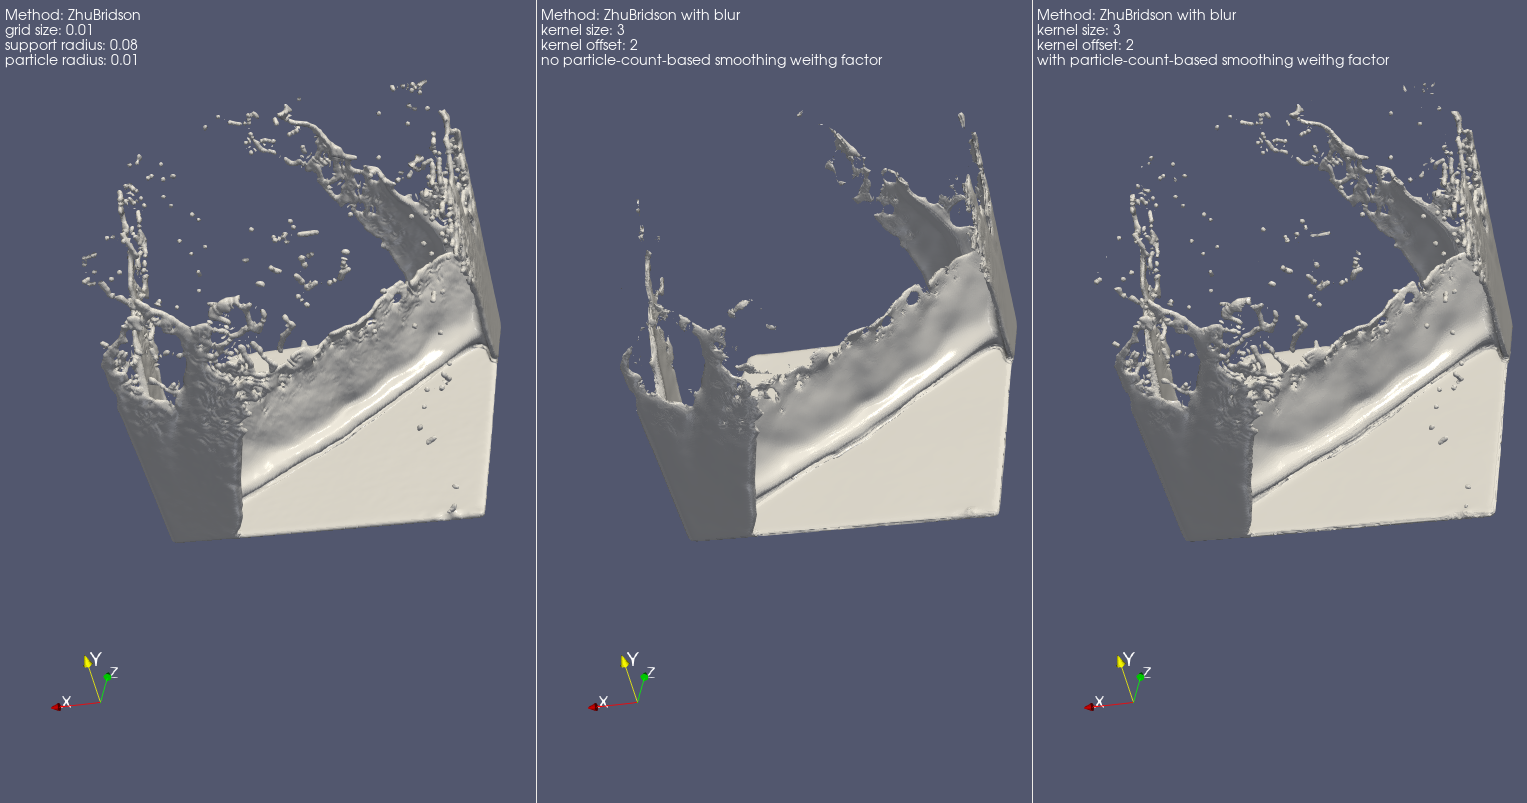
\includegraphics[width=\textwidth]{figures/View2.png}		
	\end{center}
	\caption{Leftmost is initial Zhu and Bridson reconstruction, middle - blur reconstruction w.o. smoothing factor application, rightmost - blur reconstruction with usage of smoothing factor}
	\label{fig:smoothing_factor_influence}
\end{figure}


The idea of blurring using a smoothing factor is to blur the level set as much as possible in the areas where the surface of the fluid is flat and to apply less blur in areas, where a set of MC cells lacks fluid particles. Suppose the general case in Figure \ref{fig:sf_example}. In the figure red and yellow grid, vertices contain a full and half set of particles respectively. Level set values of the grid points are supposed to be blurred as much as possible.
\begin{figure}[H]
	\begin{center}
		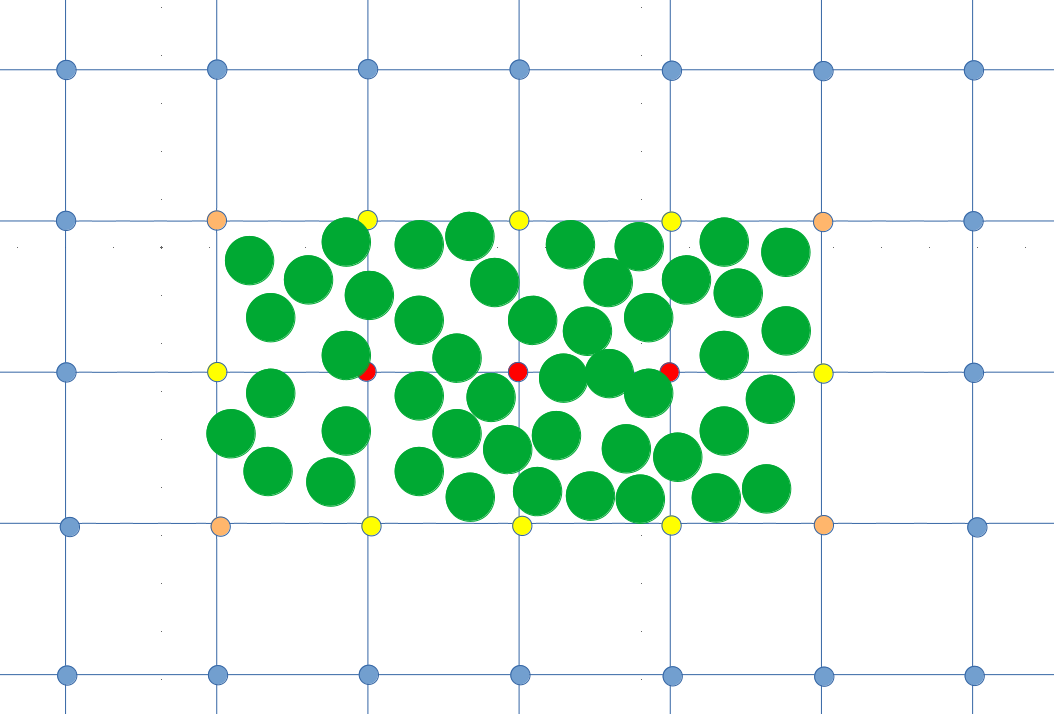
\includegraphics[width=0.5\textwidth]{figures/SmoothingFactorPictureExplenation.png}		
		\caption{Green circles are fluid particles, red - MC cells with full set of fluid particles in the neighborhood, yellow -  MC cells with half set of fluid particles in the neighborhood, orange - MC cells with quarter set of fluid particles in the neighborhood, blue - MC cells with no fluid particles in the neighborhood}
		\label{fig:sf_example}
	\end{center}
\end{figure}
Applying blur to the level set vertices that are inside the fluid (and all its neighbor cells are also inside the fluid) will not change the level set value too much as soon all vertices that has full set of fluid particles in the neighborhood will have similar level set values. 
For the MC vertices that are near the corners the 75\% of the neighbor vertices are outside the fluid, which will bias the vertex outside the fluid, thus the fluid will shrink. This is also relevant for the thin areas and splashes.\\
At the figure \ref{fig:blur_w_o_sf} the effect of surface shrinkage of applying blur in the thin area and in the corners w.r.t. the initial reconstruction method can be observed. The flat surface is smoothed out, but at the same time surface at the thin and splash areas is degraded, some small features/droplets are lost.
\begin{figure}[H]
	\begin{center}
		\begin{subfigure}[b]{\textwidth}
			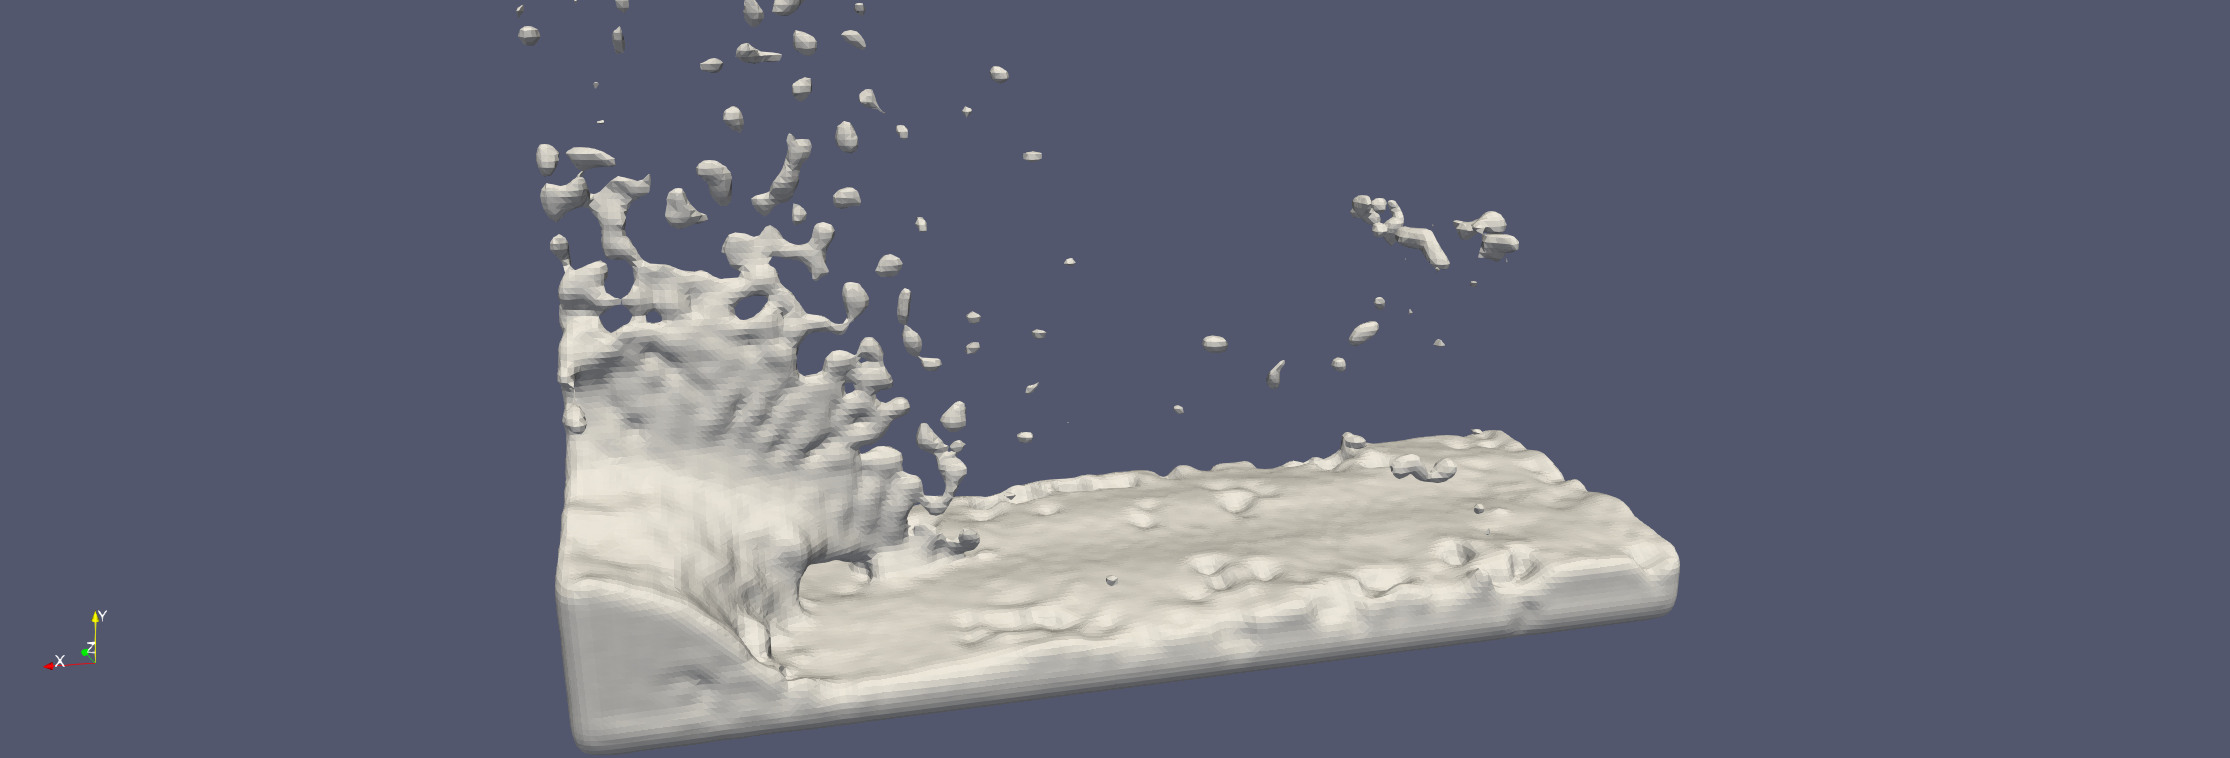
\includegraphics[width=\textwidth]{figures/DenvityBlurredSplashArea.png}
			\caption{Density based surface reconstruction}
			\label{fig:denc_rec}
		\end{subfigure}
		\begin{subfigure}[b]{\textwidth}
			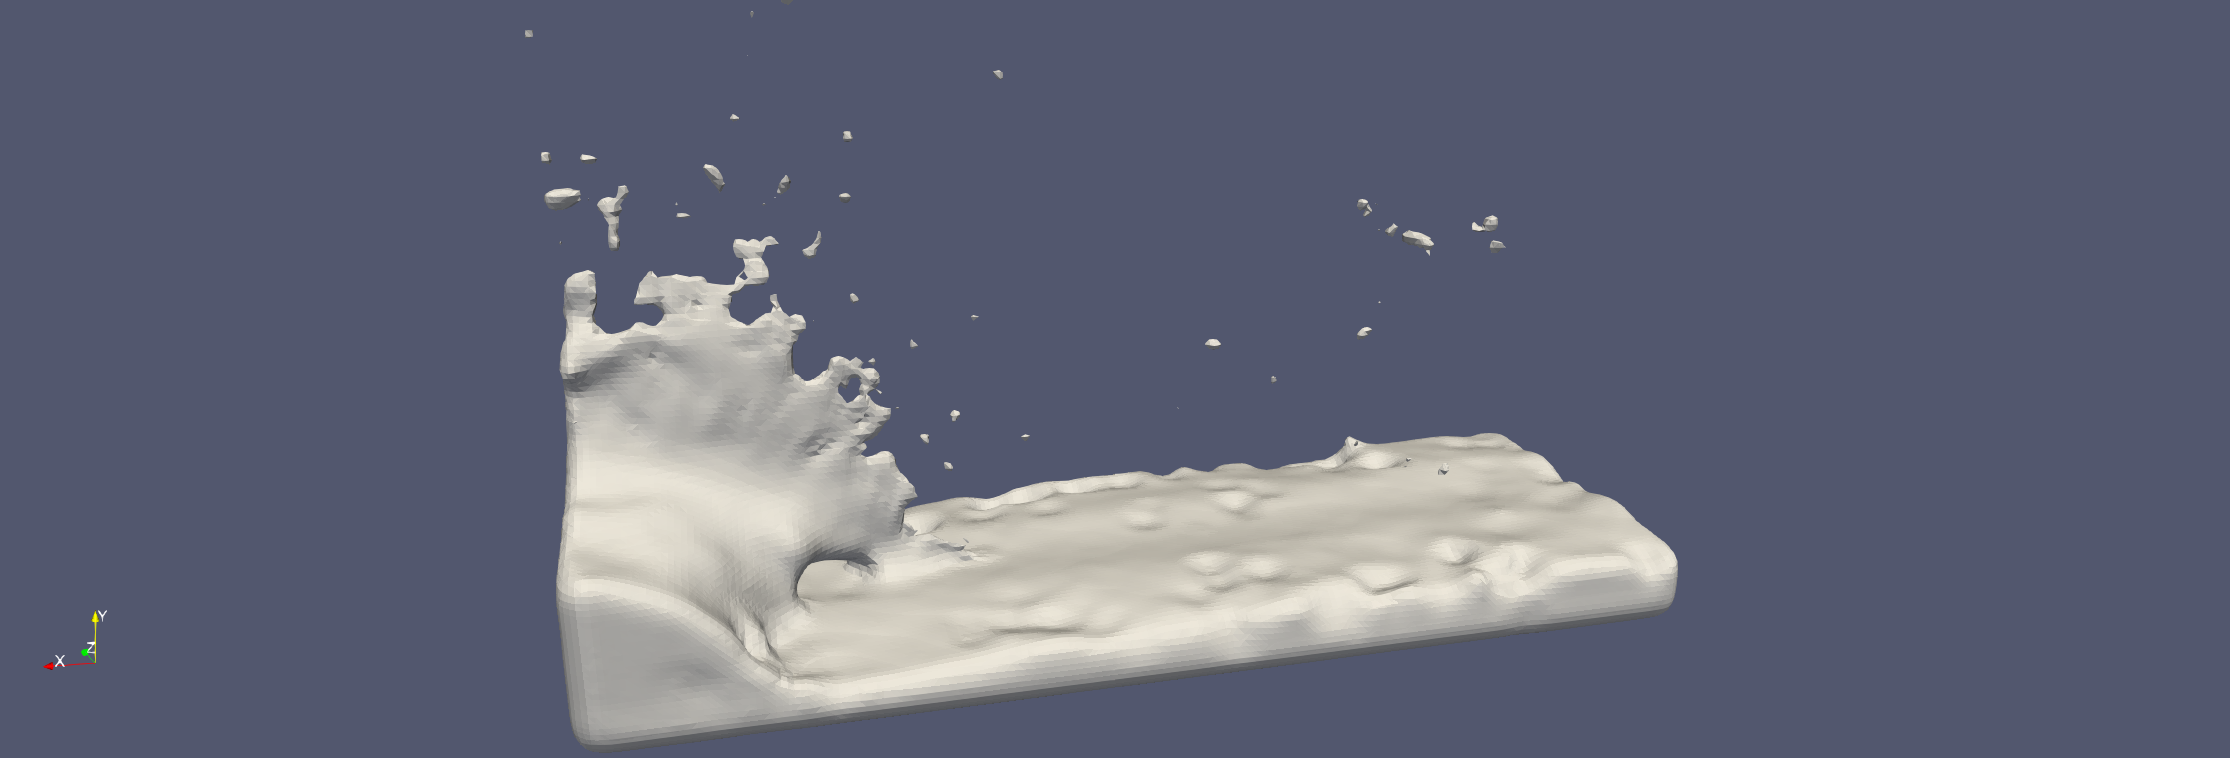
\includegraphics[width=\textwidth]{figures/DenvityBasedSplashArea.png}
			\caption{Density based surface reconstruction with blur (smoothing factor is not applied)}
			\label{fig:blur_w_o_sf}
		\end{subfigure}
	\end{center}
	\caption{Comparison of original reconstruction method and blurred reconstruction without application of smoothing factor}
	\label{fig:blur_thin_area}
\end{figure}
In the other hand applying blur on level set with smoothing factor smooths out the flat surface areas bumps, but preserves small feature areas (see Figure \label{fig:blur_thin_area_with_sf}).
\begin{figure}[H]
        \begin{subfigure}[b]{0.5\textwidth}
               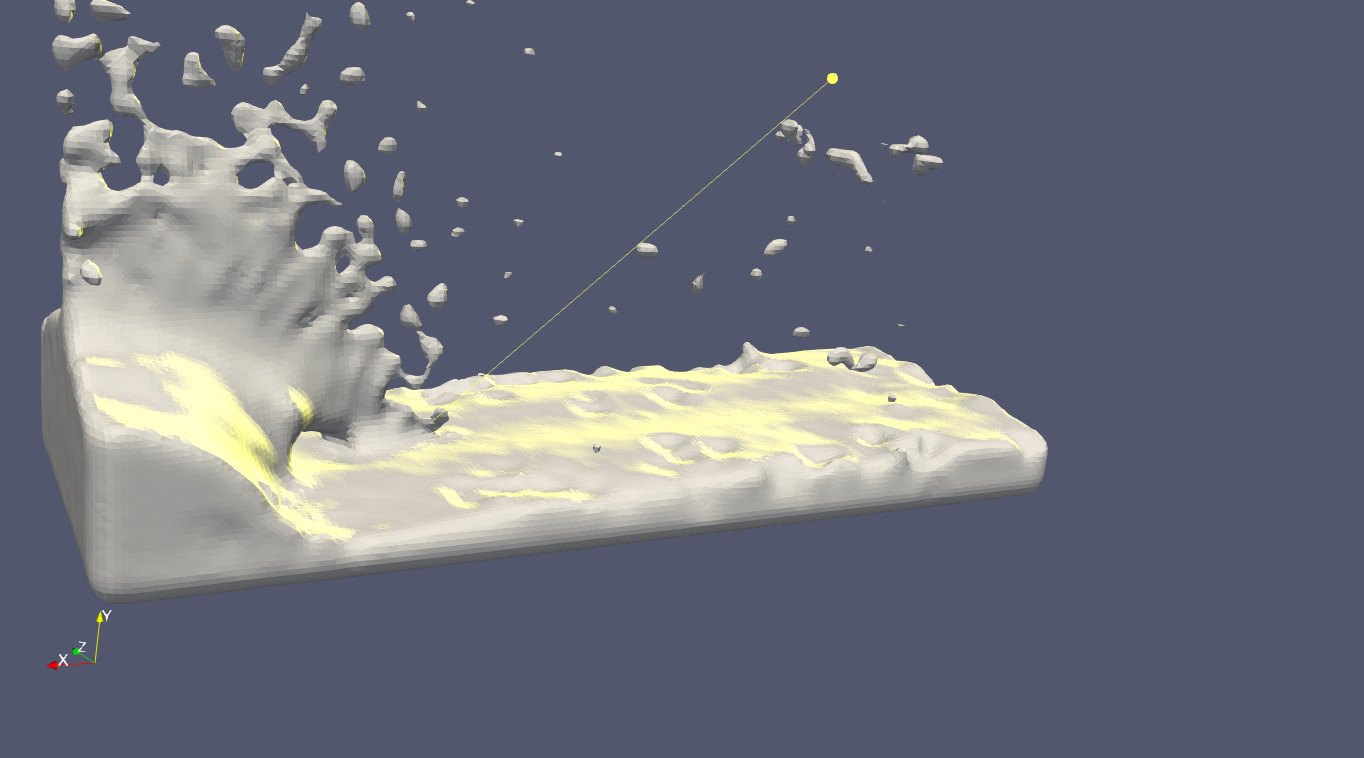
\includegraphics[width=\textwidth]{figures/DenvityBasedSplashArea2.png}
               \caption{Density based surface}
               \label{fig:db_rec}
        \end{subfigure}
        \begin{subfigure}[b]{0.5\textwidth}
               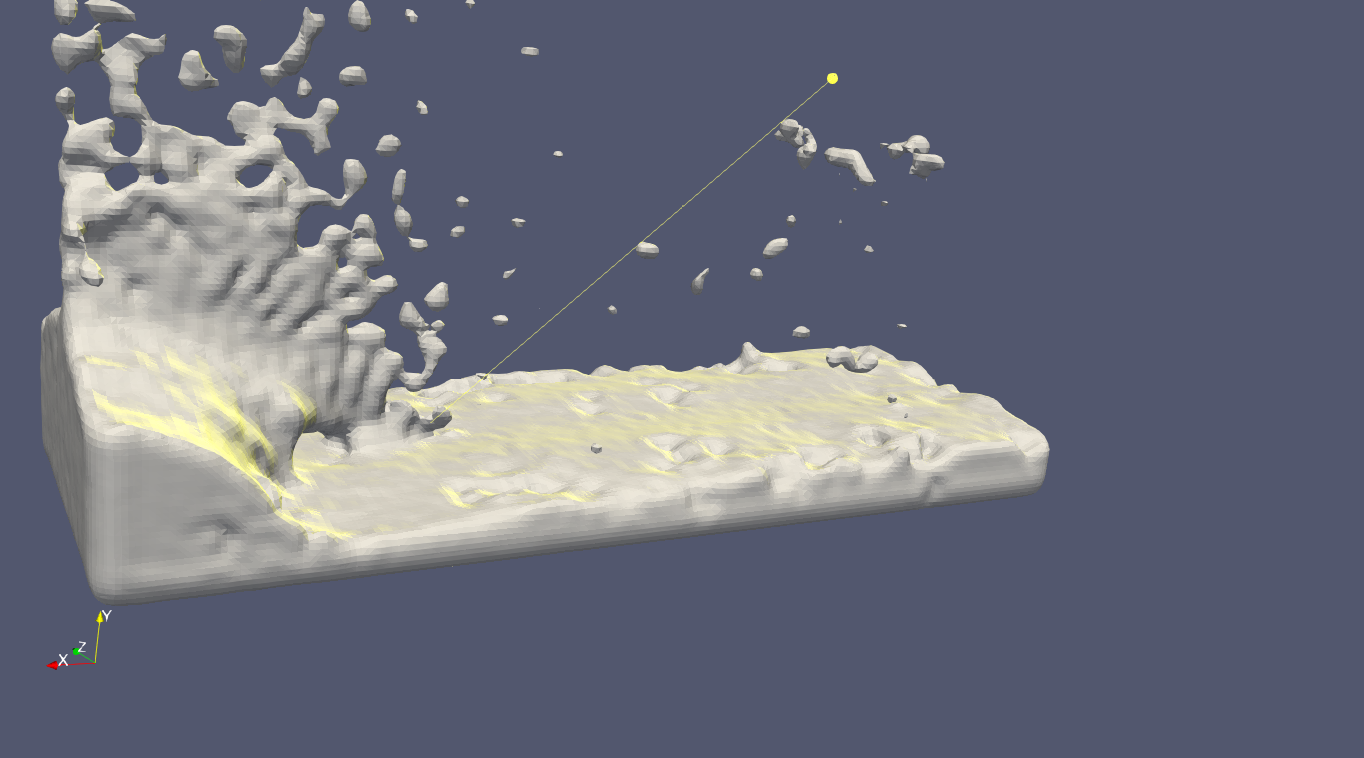
\includegraphics[width=\textwidth]{figures/DenvityBlurredSplashArea2.png}
               \caption{Applying smoothing factor to level set blur}
				\label{fig:blur_with_sf}
        \end{subfigure}
       \caption{Comparison of original reconstruction method and blurred reconstruction with application of smoothing factor}
       \label{fig:blur_thin_area_with_sf}
 \end{figure}
 \subsection{Neighbors detection algorithm}
In the Algorithm \ref{alg:blur_level_set} MC neighbor vertices are computed in function $getNeighbourVertices(vtx)$. The Algorithm \ref{alg:blur_nbs_search} describes the procedure of neighbors detection procedure.
\begin{algorithm}[H]
	\scriptsize
	\begin{algorithmic}
		\State $neighbors \gets \{\}$
		\State $sdfGradient \gets \nabla_x sdf(vtx)$
		\If{$sdfGradient \cdot sdfGradient < 1e-6$}
			\State $return\ neighbors$
		\EndIf
		\State $Normalize sdfGradient$
		
		\For{$i \in [-kernelSize \cdot kernelOffset, kernelSize \cdot kernelOffset]$, $stepsize = kernelOffset$}
			\For{$j \in [-kernelSize \cdot kernelOffset, kernelSize \cdot kernelOffset]$, $stepsize = kernelOffset$}
				\For{$k \in [-kernelSize \cdot kernelOffset, kernelSize \cdot kernelOffset]$, $stepsize = kernelOffset$}
					\If{$i = 0 \land j = 0 \land k = 0$}
						\State $neighbors \gets neighbors \cup vtx$
						\State $continue$
					\EndIf
					
					\State $offsetVector \gets [i \cdot GridResolution, j \cdot GridResolution, k \cdot GridResolution]$;
					\If{$offsetVector \cdot sdfGradient \geq kernelDepth \cdot kernelSize \cdot GridResolution$}
						\State $continue$
					\EndIf
					
					\State $neighbors \gets neighbors \cup (vtk + offsetVector)$
				\EndFor
			\EndFor
		\EndFor
		\State $return\ neighbors$
	\end{algorithmic}
	\caption{neighborhood search for level set blur algorithm}
	\label{alg:blur_nbs_search}
\end{algorithm}
The advantage of the static MC grid is that it has a static displacement of all grid vertices, thus the neighborhood can be efficiently computed. However, as it appeared, using the full neighborhood within the $kernelSize$ is not sufficient for a blur algorithm in the application to surface reconstruction. As soon as the smoothing aims to remove bumps in the flat surface areas it is more practical to take into account level set vertices, that are in the neighborhood of the fluid surface. Thus, for each vertex of the level set gradient of the level set can be computed, and the gradient vector is normal to the fluid surface \cite{LevelSetMethods}. Thus for the flat surface areas, it is convenient to blur level set vertex value w.r.t. vertices, which resides in a tangential direction to the surface normal.

\begin{figure}[H]
        \begin{subfigure}[b]{0.5\textwidth}
               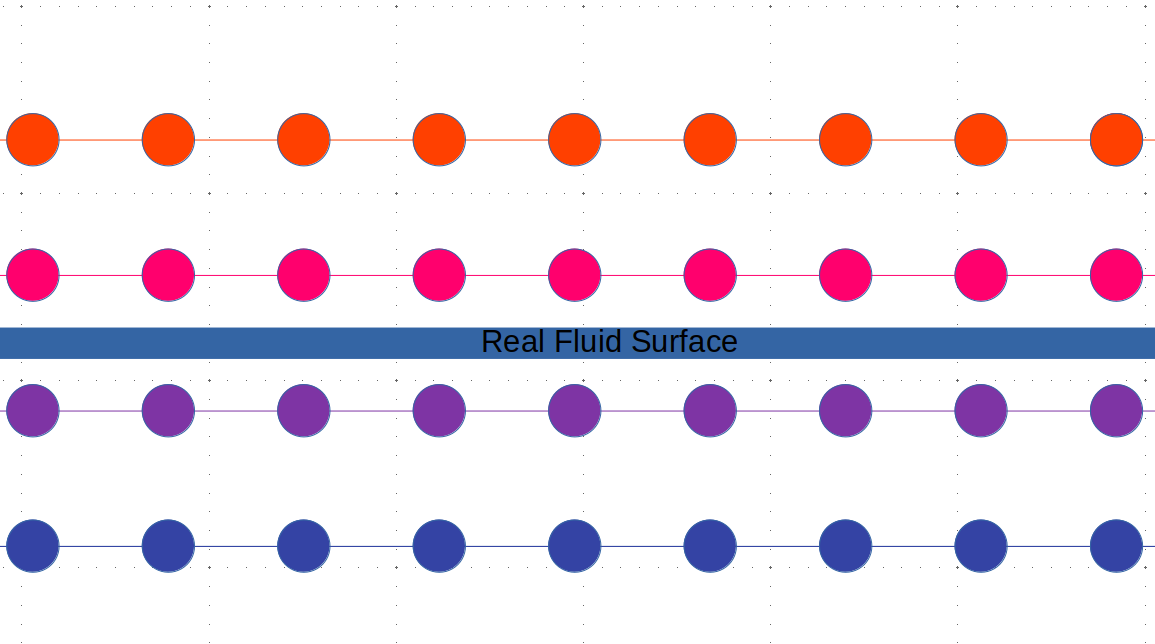
\includegraphics[width=\textwidth]{figures/RealFluidSurfaceLevelSet.png}
               \caption{Expected reconstruction of flat surface}
               \label{fig:expected_fs}
        \end{subfigure}
        \begin{subfigure}[b]{0.5\textwidth}
               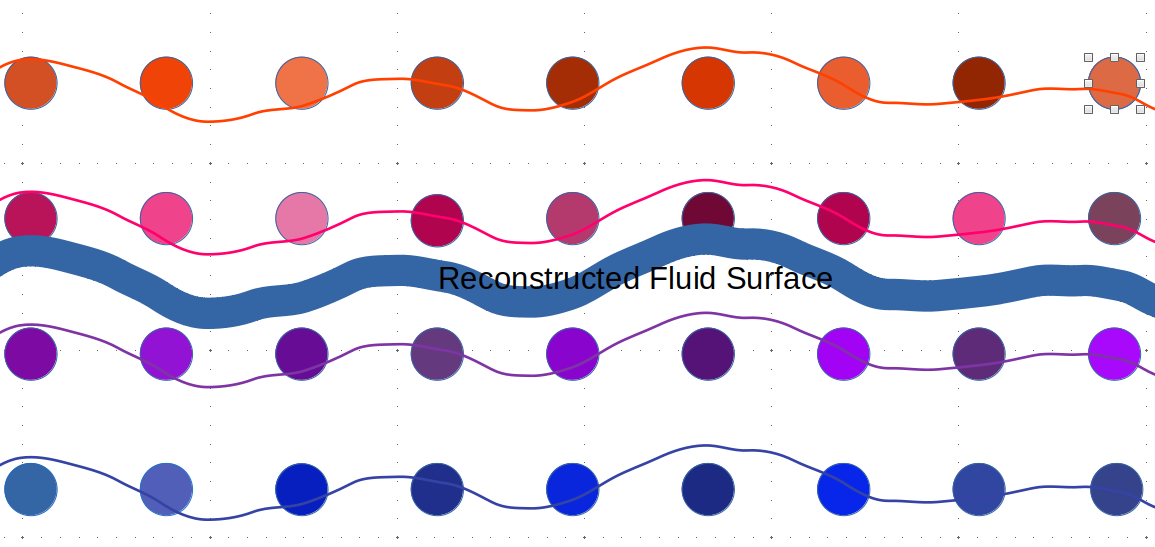
\includegraphics[width=\textwidth]{figures/ReconstructedFluidSurface.png}
               \caption{Bumpy reconstruction of flat surface}
				\label{fig:recon_fs}
        \end{subfigure}
        \begin{subfigure}[b]{0.5\textwidth}
               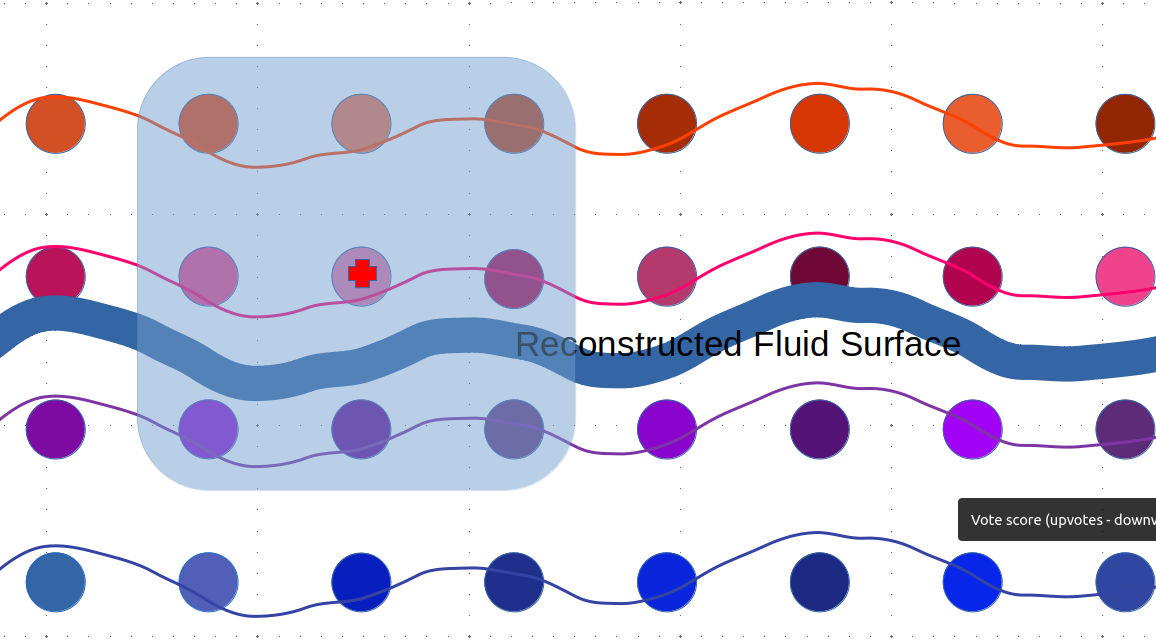
\includegraphics[width=\textwidth]{figures/LevelSetBlurFullKernel.png}
               \caption{Application of full kernel size}
               \label{fig:full_ks}
        \end{subfigure}
        \begin{subfigure}[b]{0.5\textwidth}
               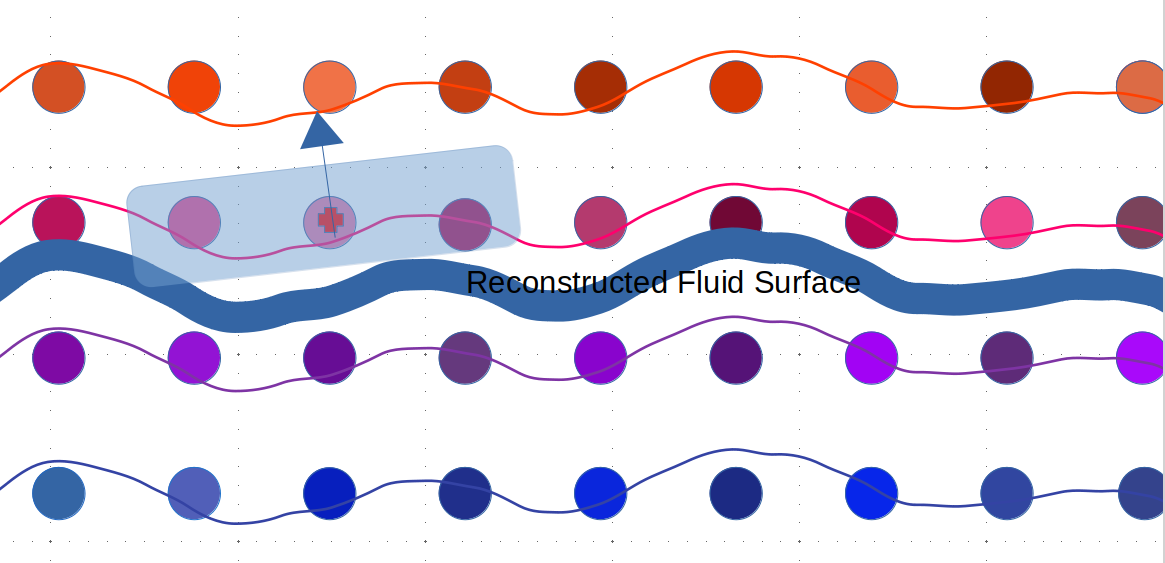
\includegraphics[width=\textwidth]{figures/LevelSetBlurKernelPart.png}
               \caption{Adjustment kernel in normal direction to iso-surface}
				\label{fig:partial_ks}
        \end{subfigure}

       \caption{Colored lines are iso-surface levels. Dots are MC grid vertices with their respective level set values}
       \label{fig:kd_surface_explenation}
 \end{figure}
At the Figure \ref{fig:expected_fs} expected fluid surface reconstruction in flat area is displayed. Dots of different colors are the MC grid vertices. Colors represent the level set value. In the perfect case level set ISO-lines (in the 2D example) forms perfect lines, thus MC grid vertices will receive similar values along the level set line. However, due to the irregular displacement of fluid particles surface is usually reconstructed as shown in Figure \ref{fig:recon_fs}. In case if we apply full kernel size (see Figure \ref{fig:full_ks}) we will pick level set values from different iso-surface levels, which will change level set values unpredictably. The better approach is to pick a kernel frame so that only level set values of near-surface MC vertices will be used for blur operation (Figure \ref{fig:partial_ks}). This way blur operation will smooth out iso-surface lines of the level set in flat regions and results in a smoother surface. Especially the influence of the kernel depth can be seen in thin areas, where kernel size is larger than a thickness of a fluid surface (see Figure \textcolor{red}{TODO: add figure}).

An example can be seen from Figure \textcolor{red}{TODO: add an example of kernel depth in real fluid domain}

\subsection{Blur kernel size and offset}
\textcolor{red}{TODO}
\section{Results}
\textcolor{red}{TODO}
\section{Performance analysis}
\textcolor{red}{TODO}
\section{Conclusions}
